\documentclass[a4paper,12pt,oneside]{book}

%------------------------------- Start of the Preable ------------------------------------------------
\usepackage[english]{babel}
\addto{\captionsenglish}{%
\renewcommand{\bibname}{References}
\renewcommand{\refname}{References}
}

\usepackage{blindtext}
\usepackage{minted}
\setcounter{secnumdepth}{3}

%\usepackage[none]{hyphenat}
\usepackage[parfill]{parskip}

\usepackage{hyperref}
\hypersetup{
    colorlinks=true,
    linkcolor=blue,
    filecolor=magenta,      
    urlcolor=cyan,
}

\urlstyle{same}
%use of package fancy header
\usepackage{fancyhdr}
\usepackage{fancyvrb}
\setlength\headheight{26pt}
\fancyhf{}
%\rhead{
\includegraphics[width=1cm]{logo}}
\lhead{\rightmark}
\rhead{
\includegraphics[width=1cm]{images/logo}}
\fancyfoot[RE, RO]{\thepage}
\fancyfoot[CE, CO]{\href{http://www.e-yantra.org}{www.e-yantra.org}}

\pagestyle{fancy}

%use of package for section title formatting
\usepackage{titlesec}
\titleformat{\chapter}
  {\Large\bfseries} % format
  {}                % label
  {0pt}             % sep
  {\huge}           % before-code
 
%use of package tcolorbox for colorful textbox
\usepackage[most]{tcolorbox}
\tcbset{colback=cyan!5!white,colframe=cyan!75!black,halign title = flush center}

\newtcolorbox{mybox}[1]{colback=cyan!5!white,
colframe=cyan!75!black,fonttitle=\bfseries,
title=\textbf{\Large{#1}}}

%use of package marginnote for notes in margin
\usepackage{marginnote}

%use of packgage watermark for pages
%\usepackage{draftwatermark}
%\SetWatermarkText{
\includegraphics{logo}}
\usepackage[scale=3.2,opacity=0.1,angle=0]{background}
\backgroundsetup{
contents={
\includegraphics{images/logo-med}}
}

%use of newcommand for keywords color
\usepackage{xcolor}
\newcommand{\keyword}[1]{\textcolor{red}{\textbf{#1}}}

%package for inserting pictures
\usepackage{graphicx}

%package for highlighting
\usepackage{color,soul}

%new command for table
\newcommand{\head}[1]{\textnormal{\textbf{#1}}}

\usepackage{dirtree}
\usepackage{siunitx}

\makeatletter
\global\let\tikz@ensure@dollar@catcode=\relax
\makeatother

\usepackage{textcomp}

%---------------------- End of the Preamble ---------------------------------------


\begin{document}

%---------------------Title Page------------------------------------------------
\begin{titlepage}
\raggedright
{\Large eYSIP 2017\\[1cm]}
{\Huge \scshape Tutorial on STM32 Programming \\[.1in]}

\vfill

\begin{figure}[!htb]
\centering
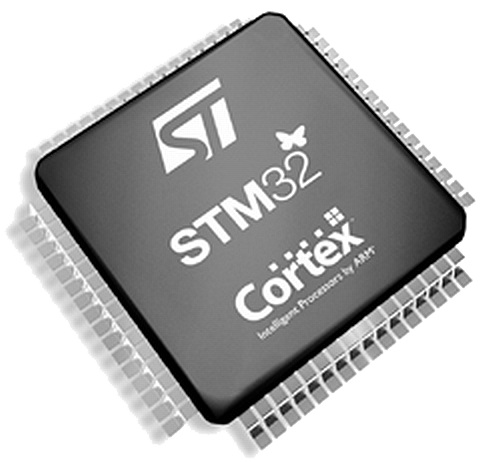
\includegraphics[width=0.7\textwidth]{images/stm32}
\end{figure}

\vfill

\begin{flushright}
{\large Heethesh Vhavle \\}
{\large Sanam Shakya \\}
{\large Pushkar Raj \\}
\vspace{0.5cm}
{\large Duration of Internship: $ 22/05/2017-07/07/2017 $ \\}
\end{flushright}
\medskip

{\itshape 2017, e-Yantra Publication}
\end{titlepage}

%-------------------------------------------------------------------------------

%\tableofcontents
%\listoffigures

%-------------------------------------------------------------------------------

\chapter[STM32 Programming]{STM32 Programming}
\section{Introduction}
The STM32 family of micro-controllers, based upon the ARM Cortex-M3 core, provides a foundation for building a vast range of embedded systems from simple battery powered dongles to complex real-time systems such as helicopter autopilots. This component family provides wide-ranging choices in memory sizes, available peripherals, performance, and power. Unfortunately, power and flexibility are achieved at a cost – software development for the STM32 family can be extremely challenging for the uninitiated with a vast array of documentation and software libraries to wade through.\cite{geob}\\

\begin{figure}[!htb]
\centering
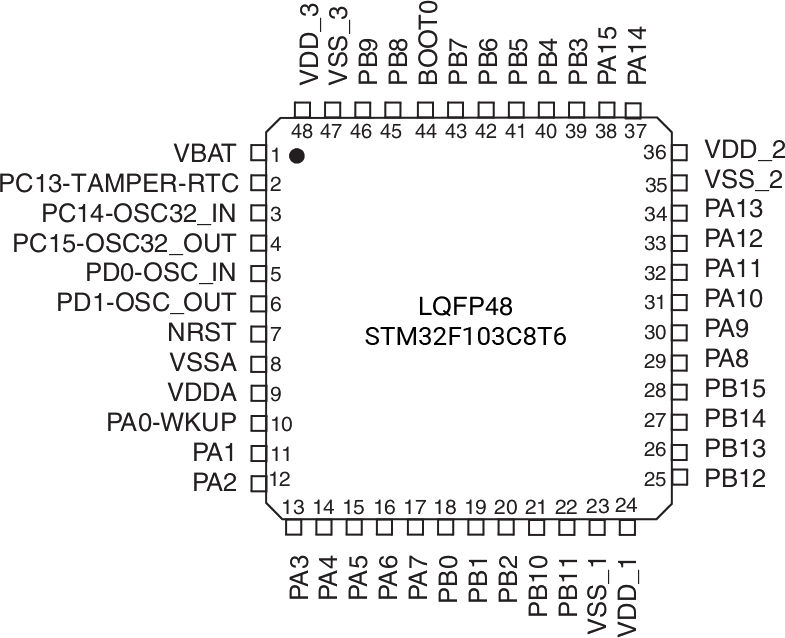
\includegraphics[width=0.7\textwidth]{images/stm32_pinout}
\caption{Pinout diagram of STM32F103C8T6 LQFP48 package}
\label{fig:stm32pin}
\end{figure}

\bigskip

The STM32F103xx medium-density performance line family incorporates the high-performance ARM Cortex-M3 32-bit RISC core operating at a 72 MHz frequency, high-speed embedded memories (Flash memory up to 128 Kbytes and SRAM up to 20 Kbytes), and an extensive range of enhanced I/Os and peripherals connected to two APB buses. All devices offer two 12-bit ADCs, three general purpose 16-bit timers plus one PWM timer, as well as standard and advanced communication interfaces: up to two I2Cs and SPIs, three USARTs, an USB and a CAN.\cite{stm32}\\

\section{List of Hardware Components}
To get started with STM32 micro-controllers, we will use the Nucleo Development board which provides an affordable and flexible way for users to try out new ideas and build prototypes. It has an on-board real-time debugger MCU called ST-LINK. This also makes the process of flashing the program easier. One can also use any other development board. Following is list of hardware choices.\\

\begin{itemize}
\item NUCLEO-F103RB STM32 Nucleo Development Board \\
\href{./datasheets/Nucleo STM32 Board.pdf}{Datasheet} | \href{./datasheets/STM32F103X.pdf}{Chip Datasheet} | \href{http://in.element14.com/stmicroelectronics/nucleo-f103rb/nucleo-board-stm32f103rbt6-mcu/dp/2394226}{Vendor Link}\\

\item STM32F103C8 Micro-controller\\
\href{./datasheets/STM32F103X.pdf}{Datasheet} | \href{./datasheets/STM32F1 Reference Manual.pdf}{Reference Manual} | \href{./datasheets/Geoffrey Brown - Discovering the STM32 Microcontroller.pdf}{Guide Book} | \href{http://www.amazon.in/STM32F103C8T6-Minimum-System-Development-Arduino/dp/B01EM11KOC/ref=sr_1_1?ie=UTF8&qid=1499069205&sr=8-1&keywords=STM32F103C8T6}{Vendor Link}\\
\end{itemize}

\section{Installation of Softwares and Tools}
This section gives a brief overview on setting up the IDE and the various methods of flashing the program on to the micro-controller. The primary software resource is the GNU software development tool-chain including gcc, objcopy, objdump, and the debugger gdb. The GNU ARM Embedded tool-chains are integrated and validated packages featuring the ARM Embedded GCC compiler, libraries and other GNU tools necessary for bare-metal software development on devices based on the ARM Cortex-M processors.\cite{geob, gnu}\\

\clearpage

\subsection{Integrated Development Environment (IDE)}
Various different options are available for choosing and IDE such as ARM Keil MDK, EWARM, TrueSTUDIO and open source options such as the Eclipse IDE. The Eclipse IDE requires the tool-chain, debug and build tools to be installed manually. The tool-chains are available for cross-compilation on Microsoft Windows, Linux and Mac OS X host operating systems. The tool-chain can be downloaded from \href{https://launchpad.net/gcc-arm-embedded/}{here}.\cite{gnu}\\

The IDE recommended for this tutorial is \href{https://atollic.com/resources/download/}{Attolic TrueSTUDIO}, which is based on the Eclipse IDE. One of the main advantages is that TrueSTUDIO IDE already comes with the GCC tool-chains for ARM and the required debugging tools.\\ 

\subsection{Debugging Tools}
\label{ssec:stmdebug}
One of the key feature of Nucleo board is that it already provides the on-chip programmer for STM32 micro-controllers. In order to use this, \href{http://www.st.com/en/embedded-software/stsw-link009.html}{ST-LINK drivers} need to be installed.\\

Although TrueSTUDIO has built-in debugging tools, some of the features are not available in the free version of the software. Instead, we can use the official \href{http://www.st.com/en/embedded-software/stsw-link004.html}{ST-LINK Utility} tool.\\

\subsection{Flashing the Program}
There are three ways to upload the firmware on to the micro-controller. One of the easiest way is to simply generate a \textit{binary (*.bin)} file, connect your board via USB and it should be detected as an external storage device. Program can be flashed by just dragging and dropping the binary file on the device.\\

The ST-LINK Utility tool also supports flashing the program on to the board. One can alternatively use the \href{http://www.amazon.in/xcluma-St-Link-Stlink-Emulator-Downloader/dp/B072TFSGW7/ref=sr_1_1?ie=UTF8&qid=1499104526&sr=8-1&keywords=st+link}{ST Link V2 Programmer}. The header for this programmer contains connections for 5V, 3.3V, SWCLK, SWDIO, SWIM, Reset (RST/NRST) and GND. The connector on the opposite side of this device is a USB connector and is intended to be plugged into the computer for programming.\\

Another method of flashing the program is by using the built-in UART Bootloader. Further details are explained \href{http://www.scienceprog.com/flashing-programs-to-stm32-embedded-bootloader/}{here}. An USART to USB driver chip like FT232 can be used along with \href{http://www.st.com/en/development-tools/flasher-stm32.html}{STM32 Flash Loader Demonstrator} to flash the program.\\ 

\section{Programming the STM32 Micro-controller}
\label{sec:progstm32}

Programming the STM32 series micro-controllers is done in various layers namely, CMSIS, HAL, BSP and Application code. The software stack is shown in \textit{\autoref{fig:software_stack}}.\\

The \textit{Cortex Micro-controller Software Interface Standard (CMSIS)} supports developers in creating reusable software components for ARM Cortex-M based systems. It mostly contains definitions for the various registers.\\

\begin{figure}[!htb]
\centering
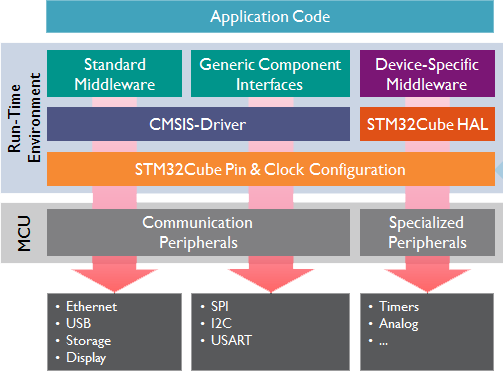
\includegraphics[width=0.75\textwidth]{images/software_stack}
\caption{Software stack for STM32 programming}
\label{fig:software_stack}
\end{figure}

The \textit{Hardware Abstraction Layer (HAL)} drivers were designed to offer a rich set of APIs and to interact easily with the application upper layers. Each driver consists of a set of functions covering the most common peripheral features such as GPIO, UART, I2C, CAN and so on.\cite{stm32hal}\\

\section{Project Setup using STM32CubeMX}
When a STM32 micro-controller starts, it needs an hardware configuration to work correctly. Unfortunately, the development of one's own HAL requires a deep knowledge of the specific micro-controller. ST provides a dedicated tool that generates the initialization code and provides us the HAL peripheral drivers. This tool is called \href{http://www.st.com/en/development-tools/stm32cubemx.html}{STM32CubeMX} and it is very useful.\cite{carmine} Let us start with a hello world project to blink a LED connected to GPIO pin.\\

\textbf{Step 1}
\medskip
\\
Open STM32CubeMX and create a \textit{New Project}. Then select the target micro-controller as \textit{STM32F103C8Tx} as shown in \textit{\autoref{fig:cube1}}.\\

\begin{figure}[!htb]
\centering
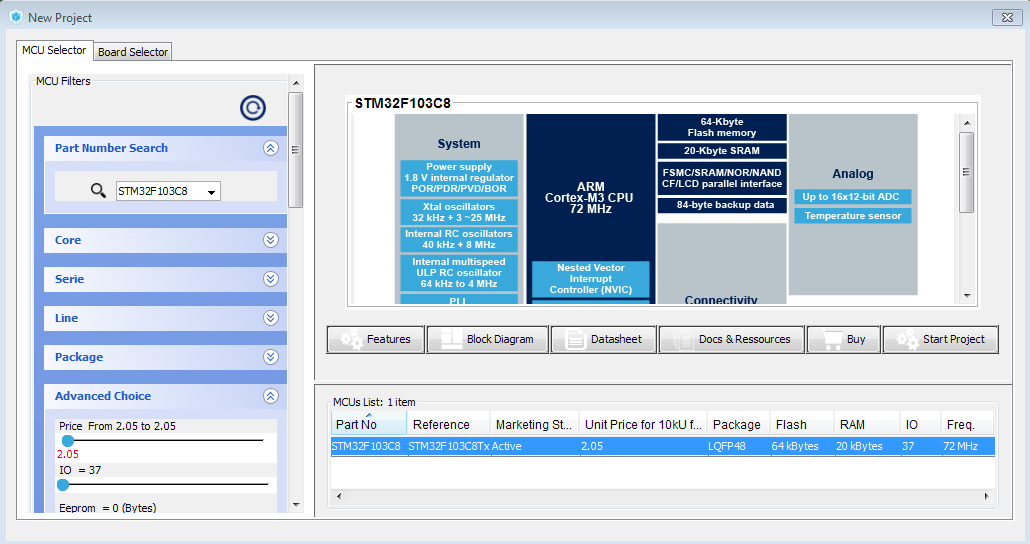
\includegraphics[width=\textwidth]{images/cubemx_1}
\caption{Selecting the target micro-controller}
\label{fig:cube1}
\end{figure}

\clearpage

\textbf{Step 2}
\medskip
\\
The micro-controller with its pinout will be displayed as shown in \textit{\autoref{fig:cube2}}. The on-board LED on Nucleo board is connected to \textit{Port A | Pin 5}. Click on \textit{PA5} and the select \textit{GPIO{\_}Output} to configure it as output pin.\\

\begin{figure}[!htb]
\centering
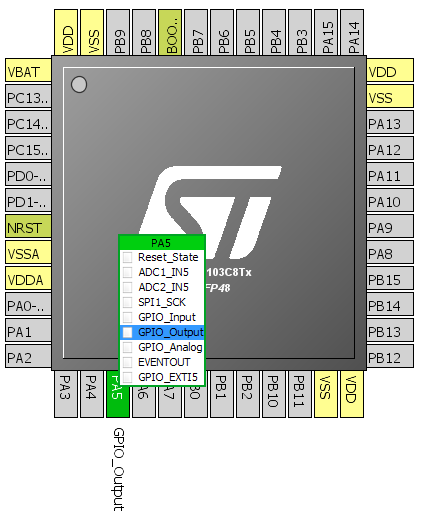
\includegraphics[width=0.8\textwidth]{images/cubemx_2}
\caption{Configuring PA5 as GPIO output pin}
\label{fig:cube2}
\end{figure}

\clearpage

\textbf{Step 3}
\medskip
\\
The next step is to configure the clock sources and set the system frequency. Click on the \textit{Clock Configuration} tab. Set HCLK as \SI{64}{\mega\hertz} as shown in \textit{\autoref{fig:cube3}}.\\

\begin{figure}[!htb]
\centering
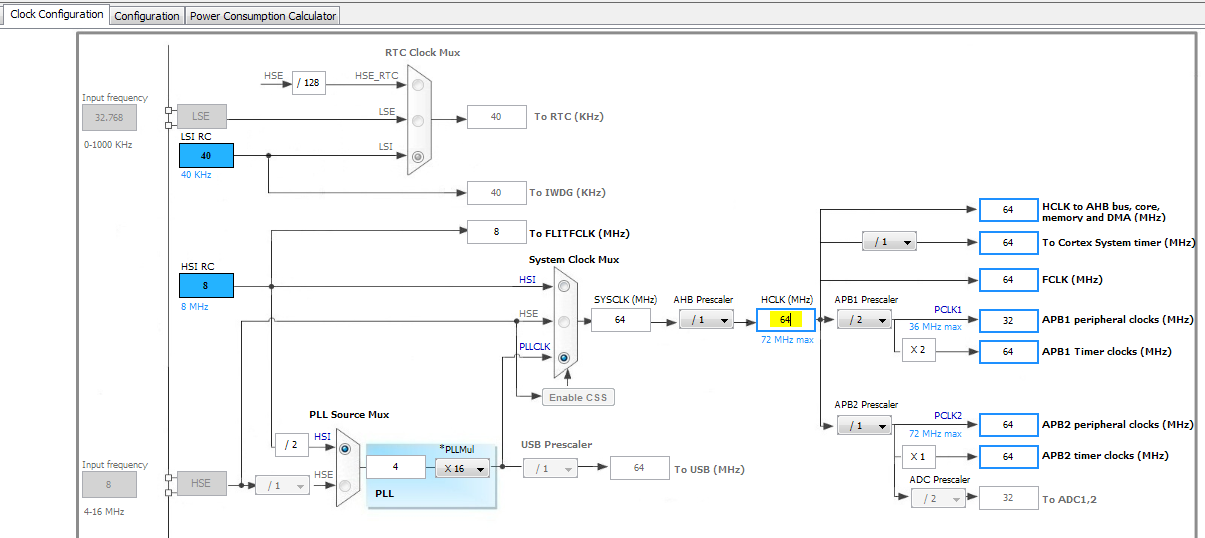
\includegraphics[width=1.2\textwidth, angle=90]{images/cubemx_3}
\caption{Configuring the clock source and system frequency}
\label{fig:cube3}
\end{figure}

\textbf{Step 4}
\medskip
\\
The final step is to generate the code and create a TrueSTUDIO project. Click the \textit{Generate source code} button as highlighted in \textit{\autoref{fig:cube4}}. The \textit{Project Settings} will open, where you configure the project name, location and the IDE. Finally, click \textit{OK} as shown in \textit{\autoref{fig:cube5}}.\\

\begin{figure}[!htb]
\centering
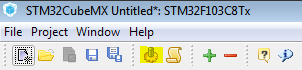
\includegraphics[width=0.5\textwidth]{images/cubemx_4}
\caption{Generate source code button}
\label{fig:cube4}
\end{figure}

\medskip

\begin{figure}[!htb]
\centering
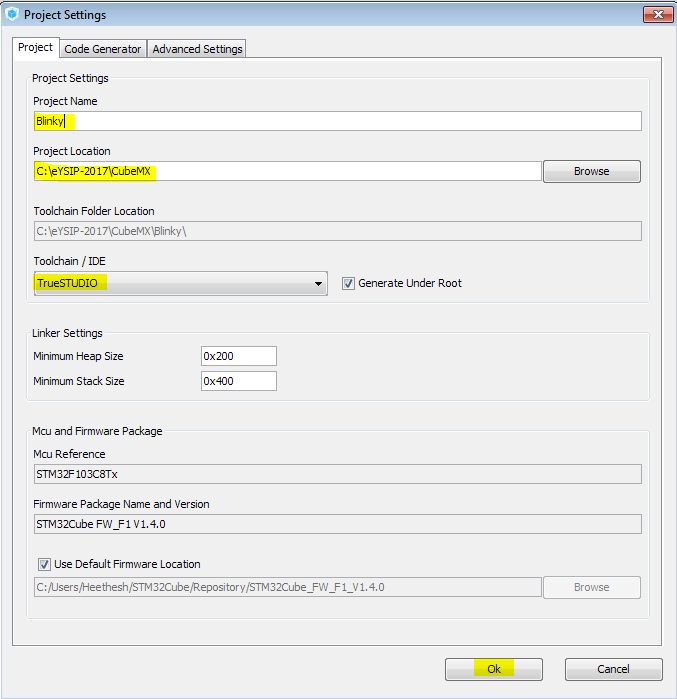
\includegraphics[width=0.8\textwidth]{images/cubemx_5}
\caption{Project settings window}
\label{fig:cube4}
\end{figure}

\section{Programming in TrueSTUDIO}
Now that the project has been setup and all the initialization is done we can begin with the programming. Open the TrueSTUDIO project file \textit{.cproject}. In the project explorer window on the left side, a bunch of folder and files created by \textit{STM32CubeMX} will be visible as shown in \textit{\autoref{fig:ts1}}.\\

\begin{figure}[!htb]
\centering
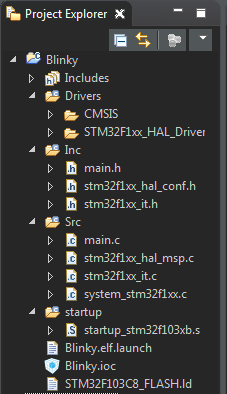
\includegraphics[width=0.4\textwidth]{images/project_tree}
\caption{Project explorer in TrueSTUDIO}
\label{fig:ts1}
\end{figure}

\bigskip

Open the \textit{main.c} file and you see the code in a template format. If you want to configure new peripherals in \textit{STM32CubeMX} along with the existing project, it will overwrite the code in the \textit{main.c} file. To prevent that from happening, various user code sections have been provided for the user to write the code and \textit{STM32CubeMX} retains this part of the code when regenerating the files next time.\\

The main function should like the snippet below. Note that the template comments have been removed here for better readability.\\

\begin{minted}[linenos=true]{c}
int main(void)
{
  /* Reset of all peripherals, Initializes the Flash 
  interface and the Systick. */
  HAL_Init();

  /* Configure the system clock */
  SystemClock_Config();

  /* Initialize all configured peripherals */
  MX_GPIO_Init();

  while (1)
  {
  }
}
\end{minted}

\bigskip
\bigskip

The HAL library provides us with functions to read, write and toggle GPIO pins. It also provides us a delay function which is based on the \textit{SysTick} counter. The default resolution of the delay function is configured to \SI{1}{\milli\second}. Following are snippets showing two different methods two blink the LED.\\

\begin{minted}[linenos=true]{c}
while (1)
{
  // Write logic HIGH to the pin
  HAL_GPIO_WritePin(GPIOA, GPIO_PIN_5, 0);
  
  // 1s delay
  HAL_Delay(1000);
  
  // Write logic LOW to the pin
  HAL_GPIO_WritePin(GPIOA, GPIO_PIN_5, 1);
  
  // 1s delay
  HAL_Delay(1000);
}
\end{minted}

\clearpage

\begin{minted}[linenos=true]{c}
while (1)
{
  // Toggle GPIO pin
  HAL_GPIO_TogglePin(GPIOA, GPIO_PIN_5);
  
  // 1s delay
  HAL_Delay(1000);
}
\end{minted}

\bigskip

The on-board LED on the Nucleo board will now blink every \SI{1}{\second}. If you are using any other development board, connect and LED to Pin A5 on the micro-controller board.\\ 

All the project files used are uploaded along with this tutorial for reference.\\

\textbf{A note on Interrupt Handlers}
\medskip
\\The \textit{stm32f1xx{\_}it.c} file in \textit{Src} folder contains the interrupt and exception handlers. The user has to implement these functions as per requirement. The \textit{SysTick} handler is also in the same file.\\

\textbf{Further reading}
\medskip
\\Geoffrey Brown's book, \href{https://www.cs.indiana.edu/~geobrown/book.pdf}{\textit{Discovering the STM32 Microcontrollers}} covers the programming on STM32 in detail. \href{http://letanphuc.net/category/stm32/}{Le Tan Phuc's blog} covers more advanced tutorials on \textit{STM32CubeMX}.\\

\begin{thebibliography}{20}
%\addcontentsline{toc}{chapter}{References}

\bibitem{geob}
Geoffrey Brown,
\href{https://www.cs.indiana.edu/~geobrown/book.pdf}{\textit{Discovering the STM32 Microcontrollers}}, 2016.

\bibitem{stm32}
STMicroelectronics, \href{http://www.st.com/content/st_com/en/products/microcontrollers/stm32-32-bit-arm-cortex-mcus/stm32f1-series/stm32f103/stm32f103rb.html}{\textit{Mainstream Performance line, ARM Cortex-M3 MCU}}.

\bibitem{gnu}
ARM Developer, \href{https://developer.arm.com/open-source/gnu-toolchain/gnu-rm}{\textit{GNU ARM Embedded Toolchain}}.

\bibitem{stm32hal}
STMicroelectronics, \href{./datasheets/STM32F1 HAL Manual.pdf}{\textit{STM32F1xx HAL Manual}}

\bibitem{carmine}
Carmine Noviello, \href{http://www.carminenoviello.com/2014/12/28/setting-gcceclipse-toolchain-stm32nucleo-part-1/}{\textit{Setting up a GCC/Eclipse toolchain for STM32Nucleo - Part 1}}

\end{thebibliography}

%-------------------------------------------------------------------

\end{document}

